\section{GPU Realization of the Shared Early-Exit Decoder}
\label{sec:cuda}

\paragraph{Question and execution boundary.}
The arithmetic saving assigned to a spatial exit map becomes useful only if
its masked decoder executes efficiently on a GPU. We therefore implemented
an opt-in inference path for the existing e15 DCVC-UF shared-exit decoder.
It changes neither checkpoint weights nor the recorded exit maps. The
six/twelve-block labels below denote exit depths \emph{within that one
e15 network}; none of the independently trained D2/D4/D6 codecs is timed
or modified here. The
measurement boundary starts with the quantized latent and decoder QP already
on the GPU and ends when the padded reconstructed tensor is ready. It
includes tile selection, shared-prefix execution, adapters, upsampling,
the output block, and grid-seam repair. It excludes analysis-transform
encoding, entropy coding/decoding, bitstream parsing, acquiring the router
map, and host-to-device transfer. A synthesis acceleration is thus distinct
from a complete decoder or complete codec acceleration.

\paragraph{Operator construction.}
The dominant DCVC-UF \texttt{DepthConvBlock} contains channel-expanding
$1\!\times\!1$ projections followed by weighted SiLU and a four-way
channel reduction. The stock PyTorch path materializes the expanded
$4C$-channel tensor and launches separate elementwise and reduction kernels.
The Triton path fuses the first projection, activation, and reduction into
one kernel that writes only $C$ channels. It also fuses the second projection
with its residual addition, and applies analogous pointwise epilogues to
the trunk, early-exit adapters, upsample boundary, and RGB head. A dedicated
depthwise kernel supports the actual replicate padding used by e15. The
full-frame seam module uses a depthwise--activation pass and one fused
pointwise--gate--residual pass. The implementation uses \texttt{tf32x3}
matrix multiplication on an RTX A6000 (SM86); inputs and outputs remain
FP32. Unsupported layout, dtype, device, or autograd conditions fall back
to the stock operators. The wrapper is installed only after checkpoint
loading and \texttt{eval()}, and converted inference weights are not saved
as training checkpoints.

\begin{figure}[t]
\centering
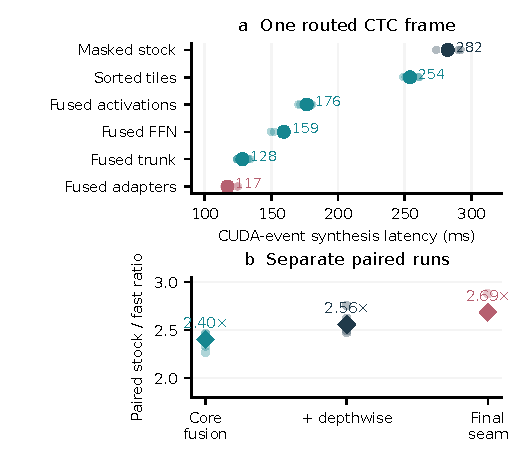
\includegraphics[width=\columnwidth]{figs/triton_20261003/latency_audit.pdf}
\caption{\textbf{An implementation gain on one real routed frame.}
\textbf{a}, Six shuffled, paired CUDA-event trials of consecutive kernel
stages. Dots are trials and large marks are medians. \textbf{b}, Three
separately timed implementations; ratios are paired \emph{within} each
run but cannot be compared as an incremental ablation across runs because
GPU contention changed. CTC videoSRC05 at QP32, $1920\times1080$ valid
pixels padded to $2048\times1280$, with exit-6/8/10/12 tile counts
13/20/4/3. The GPU was shared with training.}
\label{fig:tritongpu}
\end{figure}

\paragraph{Paired GPU measurements.}
For videoSRC05 at QP32, we replayed its archived source-calibrated router
map, containing 40 tiles and four active depths. Each six-trial block used
the same latent, QP, weights, and map, with execution order shuffled and
TF32 disabled. CUDA-event medians fell from 282.3\,ms for the stock masked
path to 254.0\,ms after depth-sorted execution, 176.5\,ms after activation
fusion, 159.3\,ms after FFN fusion, 128.2\,ms after trunk fusion, and
117.0\,ms after adapter fusion. The median of six \emph{paired} stock/fast
ratios is $2.40\times$ (individual ratios 2.27--$2.46\times$). This is a
measured synthesis gain at one map and QP, not the average speedup of the
CTC corpus.

A subsequent depthwise-enabled version gave 287.2 versus 112.1\,ms and
a median paired ratio of $2.56\times$ in four further trials on the same
frame. The host-wall medians were 289.5 and 114.6\,ms, respectively.
Adding the seam fusion produced 308.8 versus 113.3\,ms in a separate
four-trial run. The latter stock measurement drifted upward under shared
GPU load; its apparent $2.69\times$ ratio does \emph{not} establish an
incremental gain over the preceding version. A direct 16-pair seam-only
ablation within the optimized decoder measured 116.8 versus 114.8\,ms
($1.035\times$ paired median), a small contribution consistent with the
remaining whole-frame work.

\paragraph{Numerical fidelity and memory.}
The final path was checked against stock masked execution on five real
CTC frame/QP/map cases: videoSRC05 at QP 0/32/63, videoSRC01 at QP32,
and videoSRC10 at QP32. The largest absolute reconstructed-sample
difference was $6.26\times10^{-7}$; the largest absolute change in the
upstream YUV 6:1:1 PSNR was $2.09\times10^{-7}$\,dB. Tile sorting alone
was bit-exact; fused dot products are not, owing to FP32 operation order.
For the same videoSRC05 map, the incremental active-tensor allocator peak
fell from 1,069.5 to 692.1\,MB, a 35.3\% reduction. This excludes model
weights, reserved CUDA memory, and allocations held by other processes.

\paragraph{Limits and next benchmark.}
These measurements establish that the early-exit architecture can execute
substantially faster in one GPU synthesis setting, but the A6000 was not
exclusive. Other processes can change clock state, cache behaviour, and
interference between paired blocks. The 53-sequence $\times$ five-QP
benchmark is prepared with CUDA-event and wall-clock timings, checkpoint
and source hashes, and a refusal to run by default when another compute
process occupies the selected GPU. It has not been executed. The final
publication claim should come from that isolated benchmark, with
sequence-cluster uncertainty and separate QP slices, followed by an
end-to-end bitstream decode that charges entropy recovery, map signalling,
and any online router cost. The paper bundle contains the six raw GPU
records, a hash manifest, and a CPU audit script reproducing every number
in \cref{fig:tritongpu}.

\paragraph{Why one map is insufficient.}
The archived 53-sequence map inventory already shows a strong QP-dependent
workload shift: exit~6 receives 79\% of selected tiles at QP0 but 37\% at
QP63; the mean retained trunk depth rises from 6.57 to 8.24 blocks.
Different tile occupancies change the number and shape of pointwise
matmuls, gather/scatter traffic, and shared-prefix reuse. Even at the
same pixel count, one dense depth and four small occupancy groups can have
very different launch and memory behaviour. The chosen QP32 frame has
13/20/4/3 tiles at exits 6/8/10/12 and therefore probes mixed execution,
but it is not a representative-weighted CTC mean by construction. Two
small sequences lack archived maps at QP63; the prepared cohort runner
marks their dense fallback explicitly rather than silently changing the
denominator. The paper should report router-map and fallback groups
separately.

\paragraph{Rejected shortcuts.}
Several tempting local optimizations did not survive the scope check.
Pretransposing weights improved a large common-map timing by only about
0.7\%, with an additional packing cost. A separate pixel-shuffle kernel
saved only 0.024\,ms at the $2\times$ stage and had no measurable gain at
the $8\times$ output. Smaller pointwise tiles lowered register pressure,
but did not give stable whole-frame wins; the chosen FFN and pointwise
kernels use approximately 243 and 251 registers per thread, respectively,
without spills on SM86. Single-pass TF32 shortened isolated 40-tile
pointwise work by about 17--18\%, yet increased raw output error to roughly
$8\times10^{-6}$ and yielded little gain on the large common body. We
retained \texttt{tf32x3} pending a full decoder-quality sweep. None of
these microbenchmarks was promoted into the paper's speedup number.

\paragraph{Deployment accounting.}
The full codec also performs entropy recovery and may need to transmit a
mode map. An older QP32 decomposition gave separate medians of about
194.5\,ms for entropy and latent preparation and 315.0\,ms for routed
synthesis. Applying the one-frame $2.56\times$ synthesis ratio to those
older component medians would give
$(194.5+315.0)/(194.5+315.0/2.56)=1.60$ as a hypothetical total
decoder factor. Since those components were recorded at a different time
and the kernel ratio comes from one map, even this Amdahl estimate is not
a measured outcome. Future native timings must hold map acquisition and
bitstream representation fixed, report wall time alongside CUDA events,
and charge the deployment policy for its actual control overhead. This
distinguishes a faster implementation of shared early exit from a new
rate--distortion operating point.
